\section{Speculative Execution}\label{sec-haxl}

\Haxl~\citep{marlow2014haxl} is a framework for efficiently executing
code that fetches data from external sources, typically databases or
remote services. The \Haxl framework allows code written in a natural
style using \hs{Applicative} and \hs{Monad} combinators to run
efficiently, by automatically parallelising the data fetch operations
and batching together multiple fetches from the same data source.
\Haxl has been in use at Facebook, at scale, for several years now in
a system that proactively detects and remediates various forms of
abuse. \Haxl allows the engineers working on the anti-abuse code to
write clear and concise application logic, because the framework
abstracts away from the details of concurrency and efficient data fetching.

To illustrate the idea using a fragment of the example code
by~\citet{marlow2014haxl}, suppose we are writing the code to render a blog
into HTML. The blog consists of a set of posts, where each post is identified by
a \hs{PostId}. The data for the blog is stored in a remote database, and the API
for fetching the data from the database is as follows:

\vspace{1mm}
\begin{minted}[xleftmargin=10pt]{haskell}
getPostIds     :: Haxl [PostId]
getPostContent :: PostId -> Haxl PostContent
\end{minted}
\vspace{1mm}

\noindent
We can fetch the set of all \hs{PostId}s using \hs{getPostIds}, and we can fetch
the content of one post using \hs{getPostContent}. To get the content of all
posts we could write:

\vspace{0.5mm}
\begin{minted}[xleftmargin=10pt]{haskell}
getAllPostsContent :: Haxl [PostContent]
getAllPostsContent = getPostIds >>= mapM getPostContent
\end{minted}
\vspace{0.5mm}

\noindent
Now, when we \hs{mapM}~\hs{getPostContent} we would really like the
database queries to happen in parallel, because there are no
dependencies between them. Furthermore, we might even be able to batch
up the queries into a single request to the remote database.

\begin{figure}
\begin{minted}[fontsize=\small]{haskell}
-- A Haxl computation is either completed (Done) or Blocked on pending data requests
data Result a = Done a | Blocked BlockedRequests (Haxl a) deriving Functor
newtype Haxl a = Haxl { runHaxl :: IO (Result a) } deriving Functor
\end{minted}
\vspace{0mm}
\begin{minted}[fontsize=\small]{haskell}
instance Applicative Haxl where
  pure = Haxl . return . Done
  Haxl iof <*> Haxl iox = Haxl $ do
    rf <- iof
    rx <- iox
    return $ case (rf, rx) of
      (Done f      , _           ) -> f    <$> rx
      (_           , Done x      ) -> ($x) <$> rf
      (Blocked bf f, Blocked bx x) -> Blocked (bf <> bx) (f <*> x)
\end{minted}
\vspace{-13.5mm}\hspace{95mm}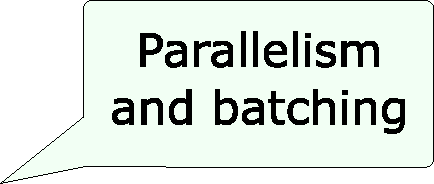
\includegraphics[scale=0.32]{fig/comment-haxl-applicative.pdf}
\vspace{3mm}
\begin{minted}[fontsize=\small]{haskell}
instance Selective Haxl where
  select (Haxl iox) (Haxl iof) = Haxl $ do
    rx <- iox
    rf <- iof
    return $ case (rx, rf) of
      (Done (Right b), _           ) -> Done b
      (Done (Left  a), _           ) -> ($a) <$> rf
      (_             , Done       f) -> either f id <$> rx
      (Blocked bx x  , Blocked bf f) -> Blocked (bx <> bf) (select x f)
\end{minted}
\vspace{-26mm}\hspace{31.5mm}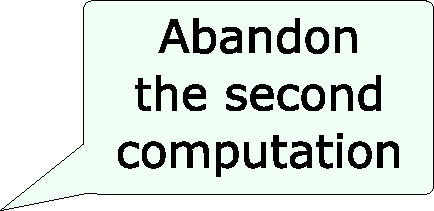
\includegraphics[scale=0.32]{fig/comment-haxl-selective-1.pdf}
\vspace{11.5mm}\hspace{110.5mm}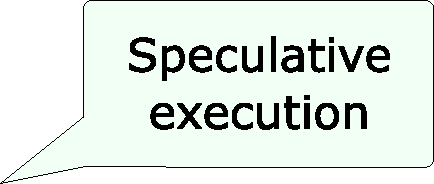
\includegraphics[scale=0.32]{fig/comment-haxl-selective-2.pdf}
\vspace{-7.5mm}
\begin{minted}[fontsize=\small]{haskell}
instance Monad Haxl where
  return = Haxl . return . Done
  Haxl iox >>= f = Haxl $ do
    rx <- iox
    case rx of Done       x -> runHaxl (f x)
               Blocked bx x -> return (Blocked bx (x >>= f))
\end{minted}
\vspace{-19mm}\hspace{31mm}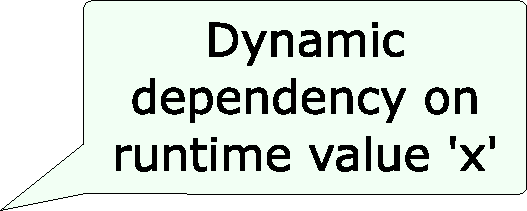
\includegraphics[scale=0.32]{fig/comment-haxl-monad.pdf}
\vspace{5mm}
\caption{An implementation of \hs{Applicative}, \hs{Selective} and \hs{Monad}
instances for the \Haxl monad.}
\label{fig-haxl}
\vspace{-3mm}
\end{figure}

These optimisations are performed automatically by \Haxl, using a
special \hs{Applicative} instance that exploits the lack of
dependency between the two computations to explore the computations
and collect the data fetch requests that can be performed in parallel or batched
together. Fig.~\ref{fig-haxl} shows an implementation adapted from the code
by~\citet{marlow2014haxl}. For the purposes of the presentation here we have
renamed \hs{Fetch} to \hs{Haxl} and omitted the exception-handling code.
The key piece of \Haxl's design is the \hs{Blocked}/\hs{Blocked} case, where
two independent sets of \hs{BlockedRequests} are combined together (the
semigroup operator \hs{<>} is just a customised set union). \Haxl also has a
\hs{Monad} instance, also shown in Fig.~\ref{fig-haxl}, which provides support
for \emph{dynamic} data fetches that are based on results obtained earlier.
Such dynamic data fetches are sequentialised as you would expect, but code
written to use \hs{Applicative} operations benefits from the automatic
concurrency. This optimisation is further exploited by using a transformation
on the monadic \cmd{do}-notation to automatically use \hs{Applicative}
operators where possible~\cite{marlow2016applicativedo}.

One of the key tools found to be useful in the kind of code written
using \Haxl at Facebook is the ``lazy'' conditional operators:

\vspace{1mm}
\begin{minted}[xleftmargin=10pt]{haskell}
(.||), (.&&) :: Haxl Bool -> Haxl Bool -> Haxl Bool
@\blk{x}@ .|| y = do b <- x; if b then return True else y
@\blk{x}@ .&& y = do b <- x; if b then y           else return False
\end{minted}
\vspace{1mm}

\noindent
These are typically used to improve performance by guarding slow
checks with faster checks.  For example, we might write:

\begin{minted}[xleftmargin=10pt]{haskell}
if simpleCondition .&& complexCondition then ... else ...
\end{minted}

\noindent
The idea is that \hs{simpleCondition} is quick to evaluate and
returns \hs{False} in a large proportion of cases, so that we can
often avoid needing to evaluate \hs{complexCondition}.

This does not require any additional extensions or special support in
\Haxl. But we also noticed that sometimes there is a pair of conditions
where neither is obviously faster than the other, yet we would still
like to benefit from bailing out early when the answer is known.
Therefore, \Haxl contains two more conditional operators \hs{pOr} and
\hs{pAnd} for ``parallel OR'' and ``parallel AND'':

\begin{minted}[xleftmargin=10pt]{haskell}
pOr, @\blu{pAnd}@ :: Haxl Bool -> Haxl Bool -> Haxl Bool
\end{minted}

\noindent
These have the behaviour that: (i)~both arguments are evaluated in parallel;
(ii)~the computation is aborted as soon as the answer is known, even if the
other argument is still being evaluated. Data fetches are not observable
effects, so the parallelism is not observable to the programmer (\Haxl relies
on this property for the soundness of its parallel \hs{Applicative}
instance). However, \hs{pOr} and \hs{pAnd} are non-deterministic with
respect to exceptions: if an exception is thrown by either side, it
will be thrown by the computation as a whole immediately without
waiting for the other side to complete.  One could imagine an
alternative implementation which waits for the completion of the other
argument when an exception is raised; this would be deterministic, but
would be less efficient in the case of exceptions.

It should come as no surprise that \hs{pOr} and \hs{pAnd} can be
implemented using \hs{select}, indeed \hs{pOr}~\hs{=}~\hs{(<||>)} and
\hs{pAnd}~\hs{=}~\hs{(<&&>)} from Fig.~\ref{fig-library}. The corresponding
\hs{Selective} instance is given in Fig.~\ref{fig-haxl}: in the
\hs{Blocked}/\hs{Blocked} case we speculatively explore both computations,
and if we obtain a \hs{Done}/\hs{Right} result, the second computation is
safely abandoned and subsequently cancelled.

There is one wrinkle with implementing \hs{pOr} and \hs{pAnd}
in terms of \hs{select}. Ideally, \hs{pOr} and \hs{pAnd} would be
symmetric: just as we can cancel the second computation if the first
one determines the answer, we should be able to cancel the first
computation in the same way. Yet \hs{select} is inherently left-biased:
it requires that all the effects of the first argument are performed.
In~\S\ref{sec-alt-symmetric} we consider an alternative combinator
related to \hs{select} that allows this kind of symmetry to be expressed.

We have prototyped an implementation of \Haxl with the \hs{Selective}~\hs{Haxl}
instance, which allowed us to reuse generic selective combinators
\hs{<||>}, \hs{<&&>}, \hs{anyS} and \hs{allS} instead of providing custom
implementations for conditional operators \hs{pOr} and \hs{pAnd} and
their generalisations on lists. This case study highlights the fact that
selective functors are useful not only in the static context, but in the dynamic
context too, by allowing us to benefit from speculative execution.

\subsection{Results}

We mentioned above that \hs{pOr} and \hs{pAnd} are effective when the
relative size of the conditional computations is unknown, so
evaluating them in parallel with early exit is an effective
alternative to either sequencing them manually (with \hs{Monad}) or
evaluating them in parallel to completion (with
\hs{Applicative}). This argument becomes even more compelling as the
set of conditions to evaluate grows: imagine trying to efficiently
sequence a set of ten or more conditions, and then repeating the
exercise every time the set changes.

For this reason, in \Haxl we found that list operations built on top
of \hs{pOr} and \hs{pAnd}, which in this paper we call \hs{anyS} and
\hs{allS} (see Fig.~\ref{fig-library}), offer an important balance
between performance and maintainability that is not provided by the
\hs{Applicative} or \hs{Monad}-based combinators.

One could construct examples to demonstrate arbitrarily large
performance gains from using \hs{pOr} and \hs{pAnd}, however that
would not be particularly useful. Perhaps more useful would be a
real-world measurement showing how much performance was improved in an
actual application but again, the value of that would depend to a
large extent on how the application uses \hs{pOr} and \hs{pAnd}, and
unfortunately the application code in our case is
proprietary. Therefore instead we offer this anecdote: we first
introduced a use of \hs{pOr} to solve some performance issues in a
complex production workload where we had long chains of conditionals
that were difficult to optimise by hand, and \hs{pOr} resulted in
significant performance improvements.
